% =============================================================
% DPCN Assignment 1: Opinion Network Formation -- Report Template
% Compile with: pdflatex report.tex  (run twice if you add refs/TOC)
%
% This is a SKELETON: headings/subheadings give the required
% structure and direction; you fill in the actual content.
% Section order below matches the assignment brief exactly --
% do not reorder.
%
% Suggested page budget (target: 8 pages total):
%   Common material (Team Name, GitHub Link, Dataset Documentation,
%   Results and Discussion, Individual Contribution)        ~2 pages
%   Each member's own content -- their subsection in
%   Section 4 (Pipeline Followed) + their subsection in
%   Section 5 (Analysis and Visualizations) combined         ~2 pages/person
%   3 members x 2 pages + 2 common pages = 8 pages total
% Keep figures compact (place related figures side by side at
% ~0.45-0.5\textwidth each rather than stacked full-width) so one
% person's 2-page budget isn't eaten by oversized diagrams.
% =============================================================
\documentclass[11pt]{article}

\usepackage[margin=1in]{geometry}
\usepackage{graphicx}
\usepackage{booktabs}
\usepackage{caption}
\usepackage{amsmath}
\usepackage{enumitem}
\usepackage{xcolor}
\usepackage{tikz}
\usetikzlibrary{arrows.meta, positioning}
\usepackage{hyperref}
\hypersetup{colorlinks=true, linkcolor=blue, urlcolor=blue, citecolor=blue}

\setlength{\parskip}{0.5em}
\setlength{\parindent}{0em}

\title{\vspace{-1.5em}Opinion Network Formation\\
\large Assignment 1: LinkedOut}
\date{\today}

\begin{document}
\maketitle
\vspace{-2em}

% -----------------------------------------------------------------
\section{Team Name}
% -----------------------------------------------------------------
\textbf{LinkedOut}

\begin{itemize}[nosep]
    \item Priyanka Agarwal (Roll No.\ 2024101016)
\end{itemize}

% -----------------------------------------------------------------
\section{GitHub Link to Code}
% -----------------------------------------------------------------
Repository: \url{https://github.com/dawnbliss-coder/opinion-network-formation}

% -----------------------------------------------------------------
\section{Dataset Documentation}
% -----------------------------------------------------------------

\subsection{Data Description}

\subsection{Encoding and Preprocessing}

\subsection{Handling Missing Data and Data Quality}

% -----------------------------------------------------------------
\section{Pipeline Followed}
% -----------------------------------------------------------------

\subsection{User--User Network}

\subsection{Statement--Statement Network}

\subsection{User--Statement Network}

\begin{figure}[h]
\centering
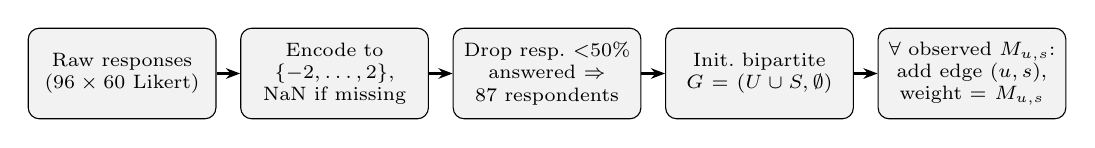
\begin{tikzpicture}[
  block/.style={rectangle, draw, fill=gray!10, rounded corners, text width=2.15cm,
                align=center, minimum height=1.15cm, font=\scriptsize},
  arrow/.style={thick, -{Stealth[length=1.8mm]}}
]
\node[block] (raw) {Raw responses\\($96\times 60$ Likert)};
\node[block, right=0.3cm of raw] (encode) {Encode to\\$\{-2,\dots,2\}$,\\NaN if missing};
\node[block, right=0.3cm of encode] (filter) {Drop resp.\ $<$50\%\\answered $\Rightarrow$\\87 respondents};
\node[block, right=0.3cm of filter] (graph) {Init.\ bipartite\\$G=(U\cup S,\emptyset)$};
\node[block, right=0.3cm of graph] (edges) {$\forall$ observed $M_{u,s}$:\\add edge $(u,s)$,\\weight $=M_{u,s}$};
\draw[arrow] (raw) -- (encode);
\draw[arrow] (encode) -- (filter);
\draw[arrow] (filter) -- (graph);
\draw[arrow] (graph) -- (edges);
\end{tikzpicture}
\caption{User--Statement network construction pipeline.}
\label{fig:pipeline-flow}
\end{figure}

Formally, let $M \in \{-2,-1,0,1,2,\mathrm{NaN}\}^{U \times S}$ be the encoded, engagement-filtered
response matrix ($|U|{=}87$ respondents, $|S|{=}60$ statements). The network is the bipartite graph
$G=(U \cup S, E)$ with $(u,s) \in E \iff M_{u,s}$ is observed (not NaN), and edge weight
$w_{u,s} = M_{u,s} \in \{-2,-1,0,1,2\}$. No edge is created for a skipped/``No Comments'' entry, since
skipping $\neq$ a Neutral (0) response.

A reference check (\texttt{edge\_threshold\_table()} in \texttt{src/user\_statement\_network.py})
confirms that sparsifying by response magnitude does not produce a meaningfully sparser graph:

\begin{center}
\small
\begin{tabular}{lcc}
\toprule
\textbf{Cutoff} & \textbf{Edges} & \textbf{Density} \\
\midrule
All answered (incl.\ Neutral) & 5{,}158 & 98.8\% \\
Drop Neutral only             & 4{,}491 & 86.0\% \\
Strongly Agree/Disagree only  & 2{,}349 & 45.0\% \\
\bottomrule
\end{tabular}
\end{center}

% -----------------------------------------------------------------
\section{Analysis and Visualizations}
% -----------------------------------------------------------------

\subsection{User--User Network}

\subsection{Statement--Statement Network}

\subsection{User--Statement Network}

\begin{figure}[h]
    \centering
    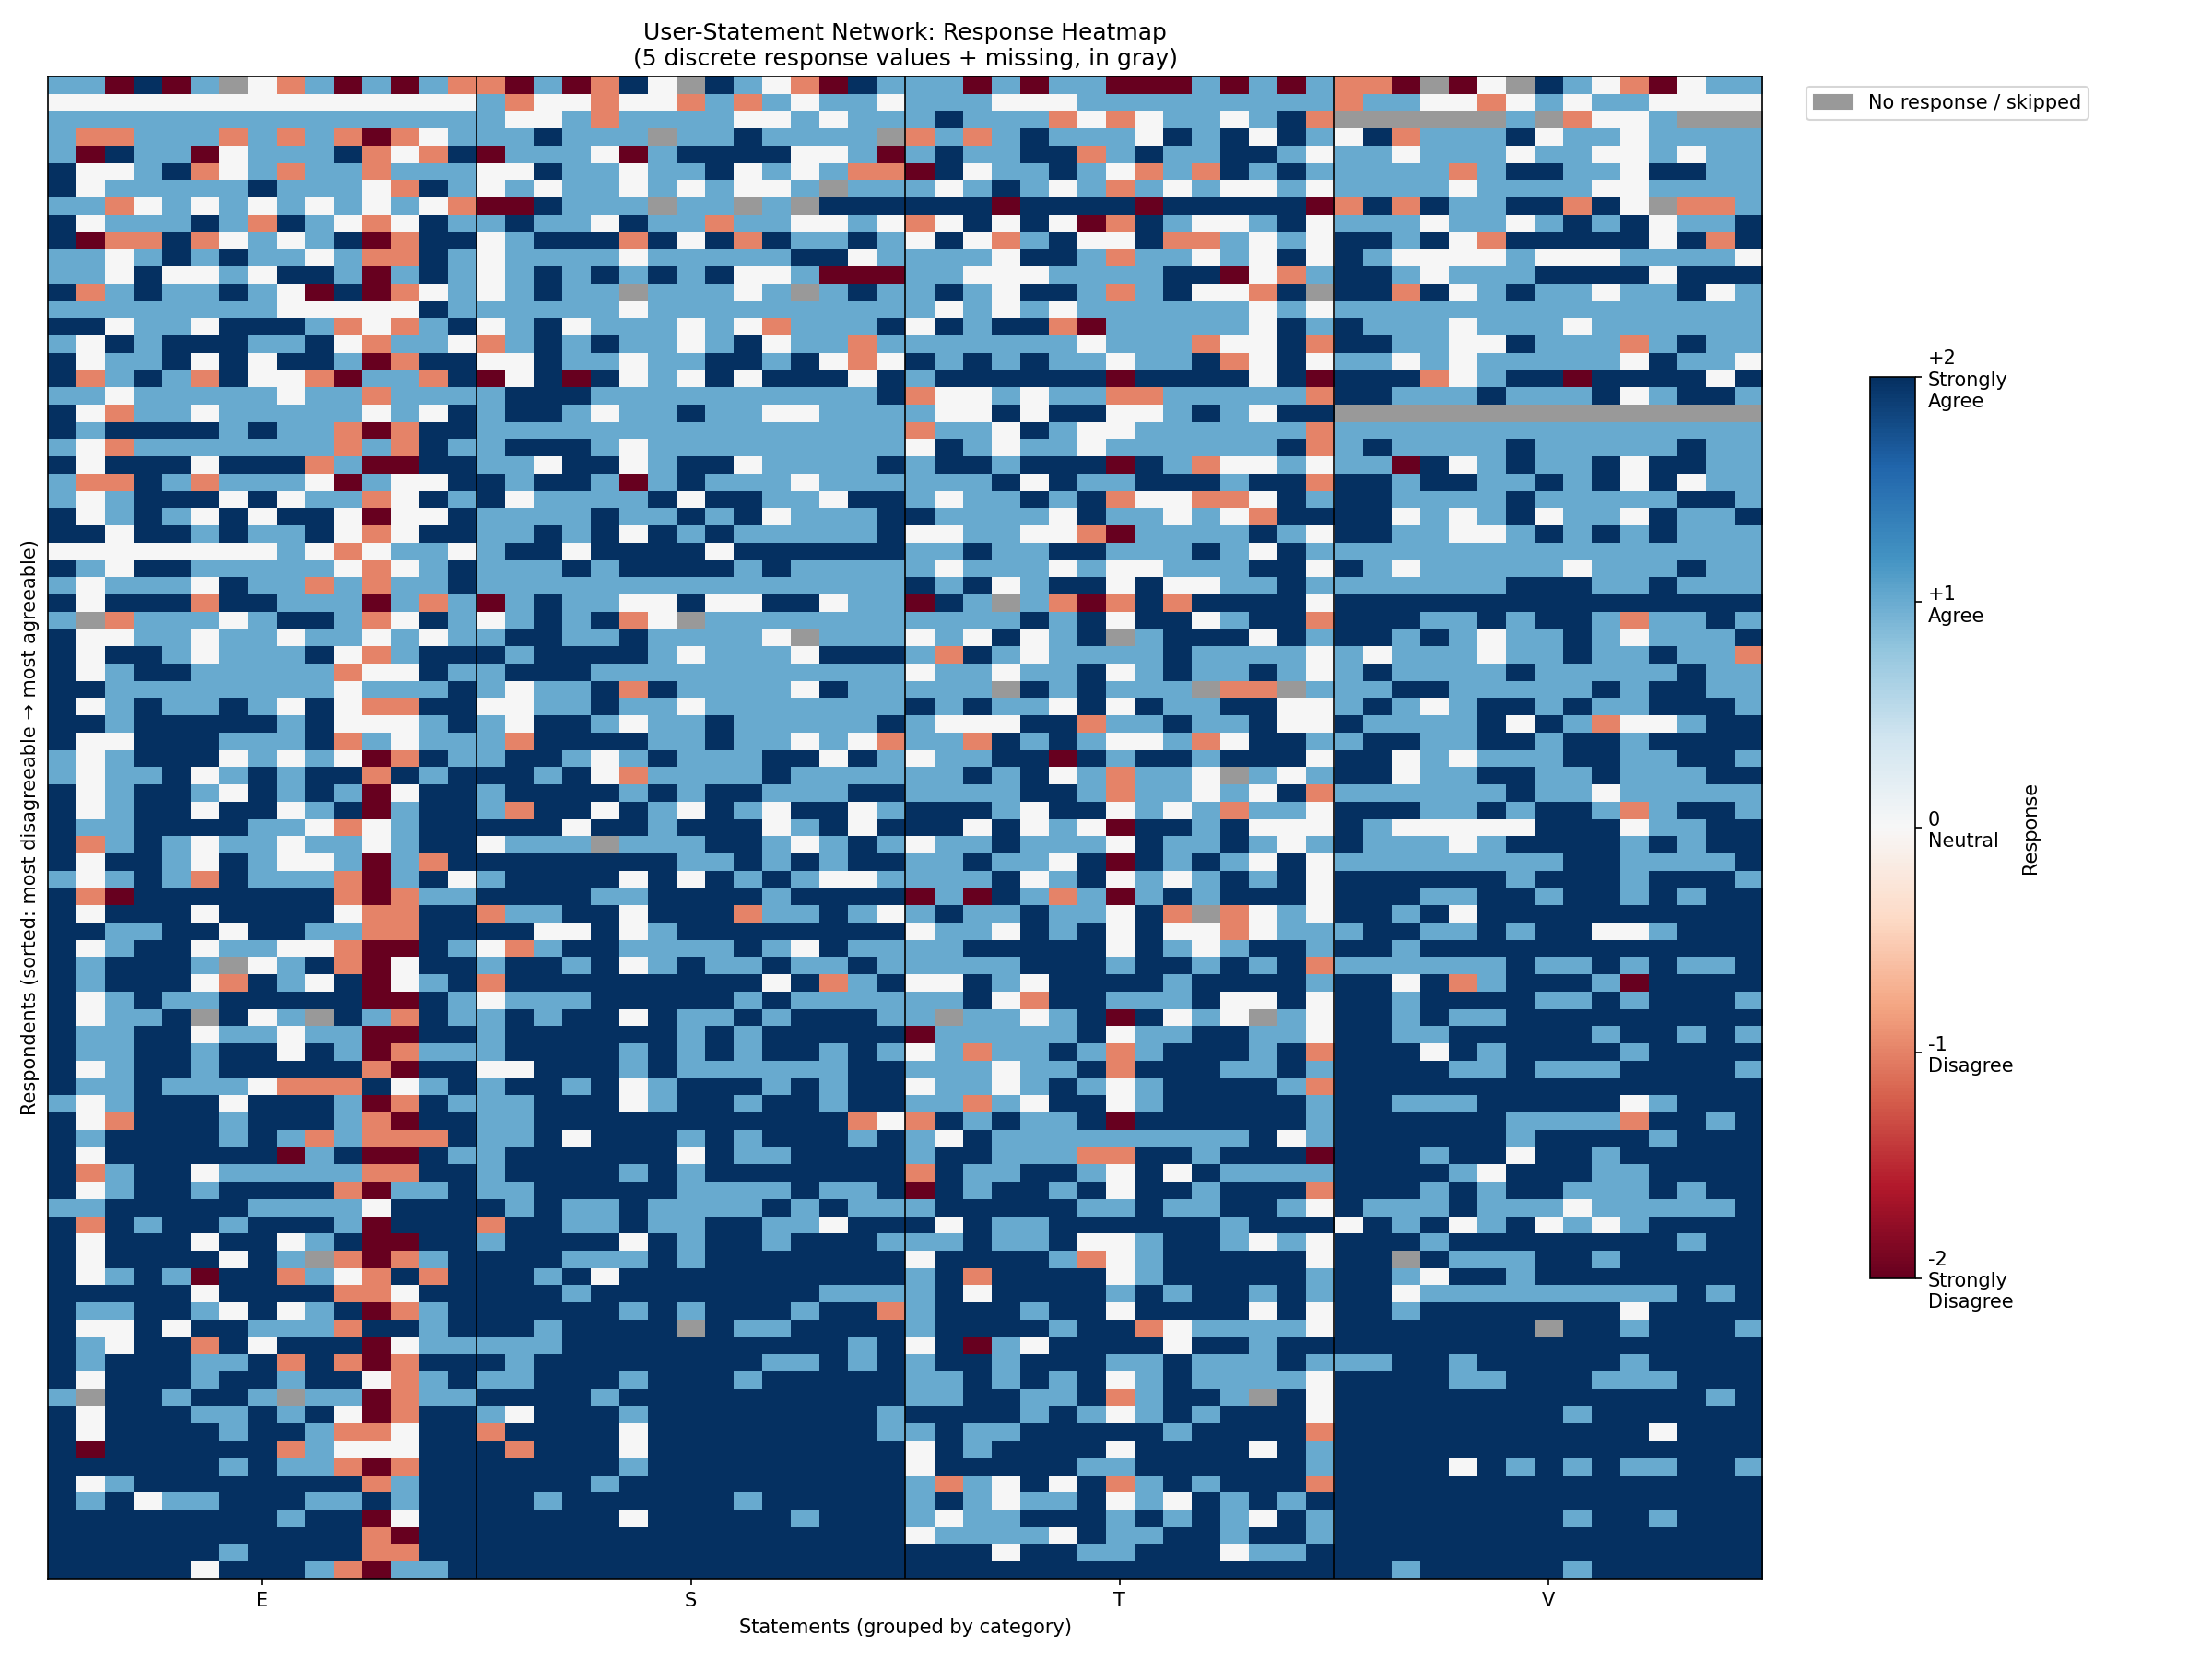
\includegraphics[width=0.47\textwidth]{../figures/user_statement_heatmap.png}\hfill
    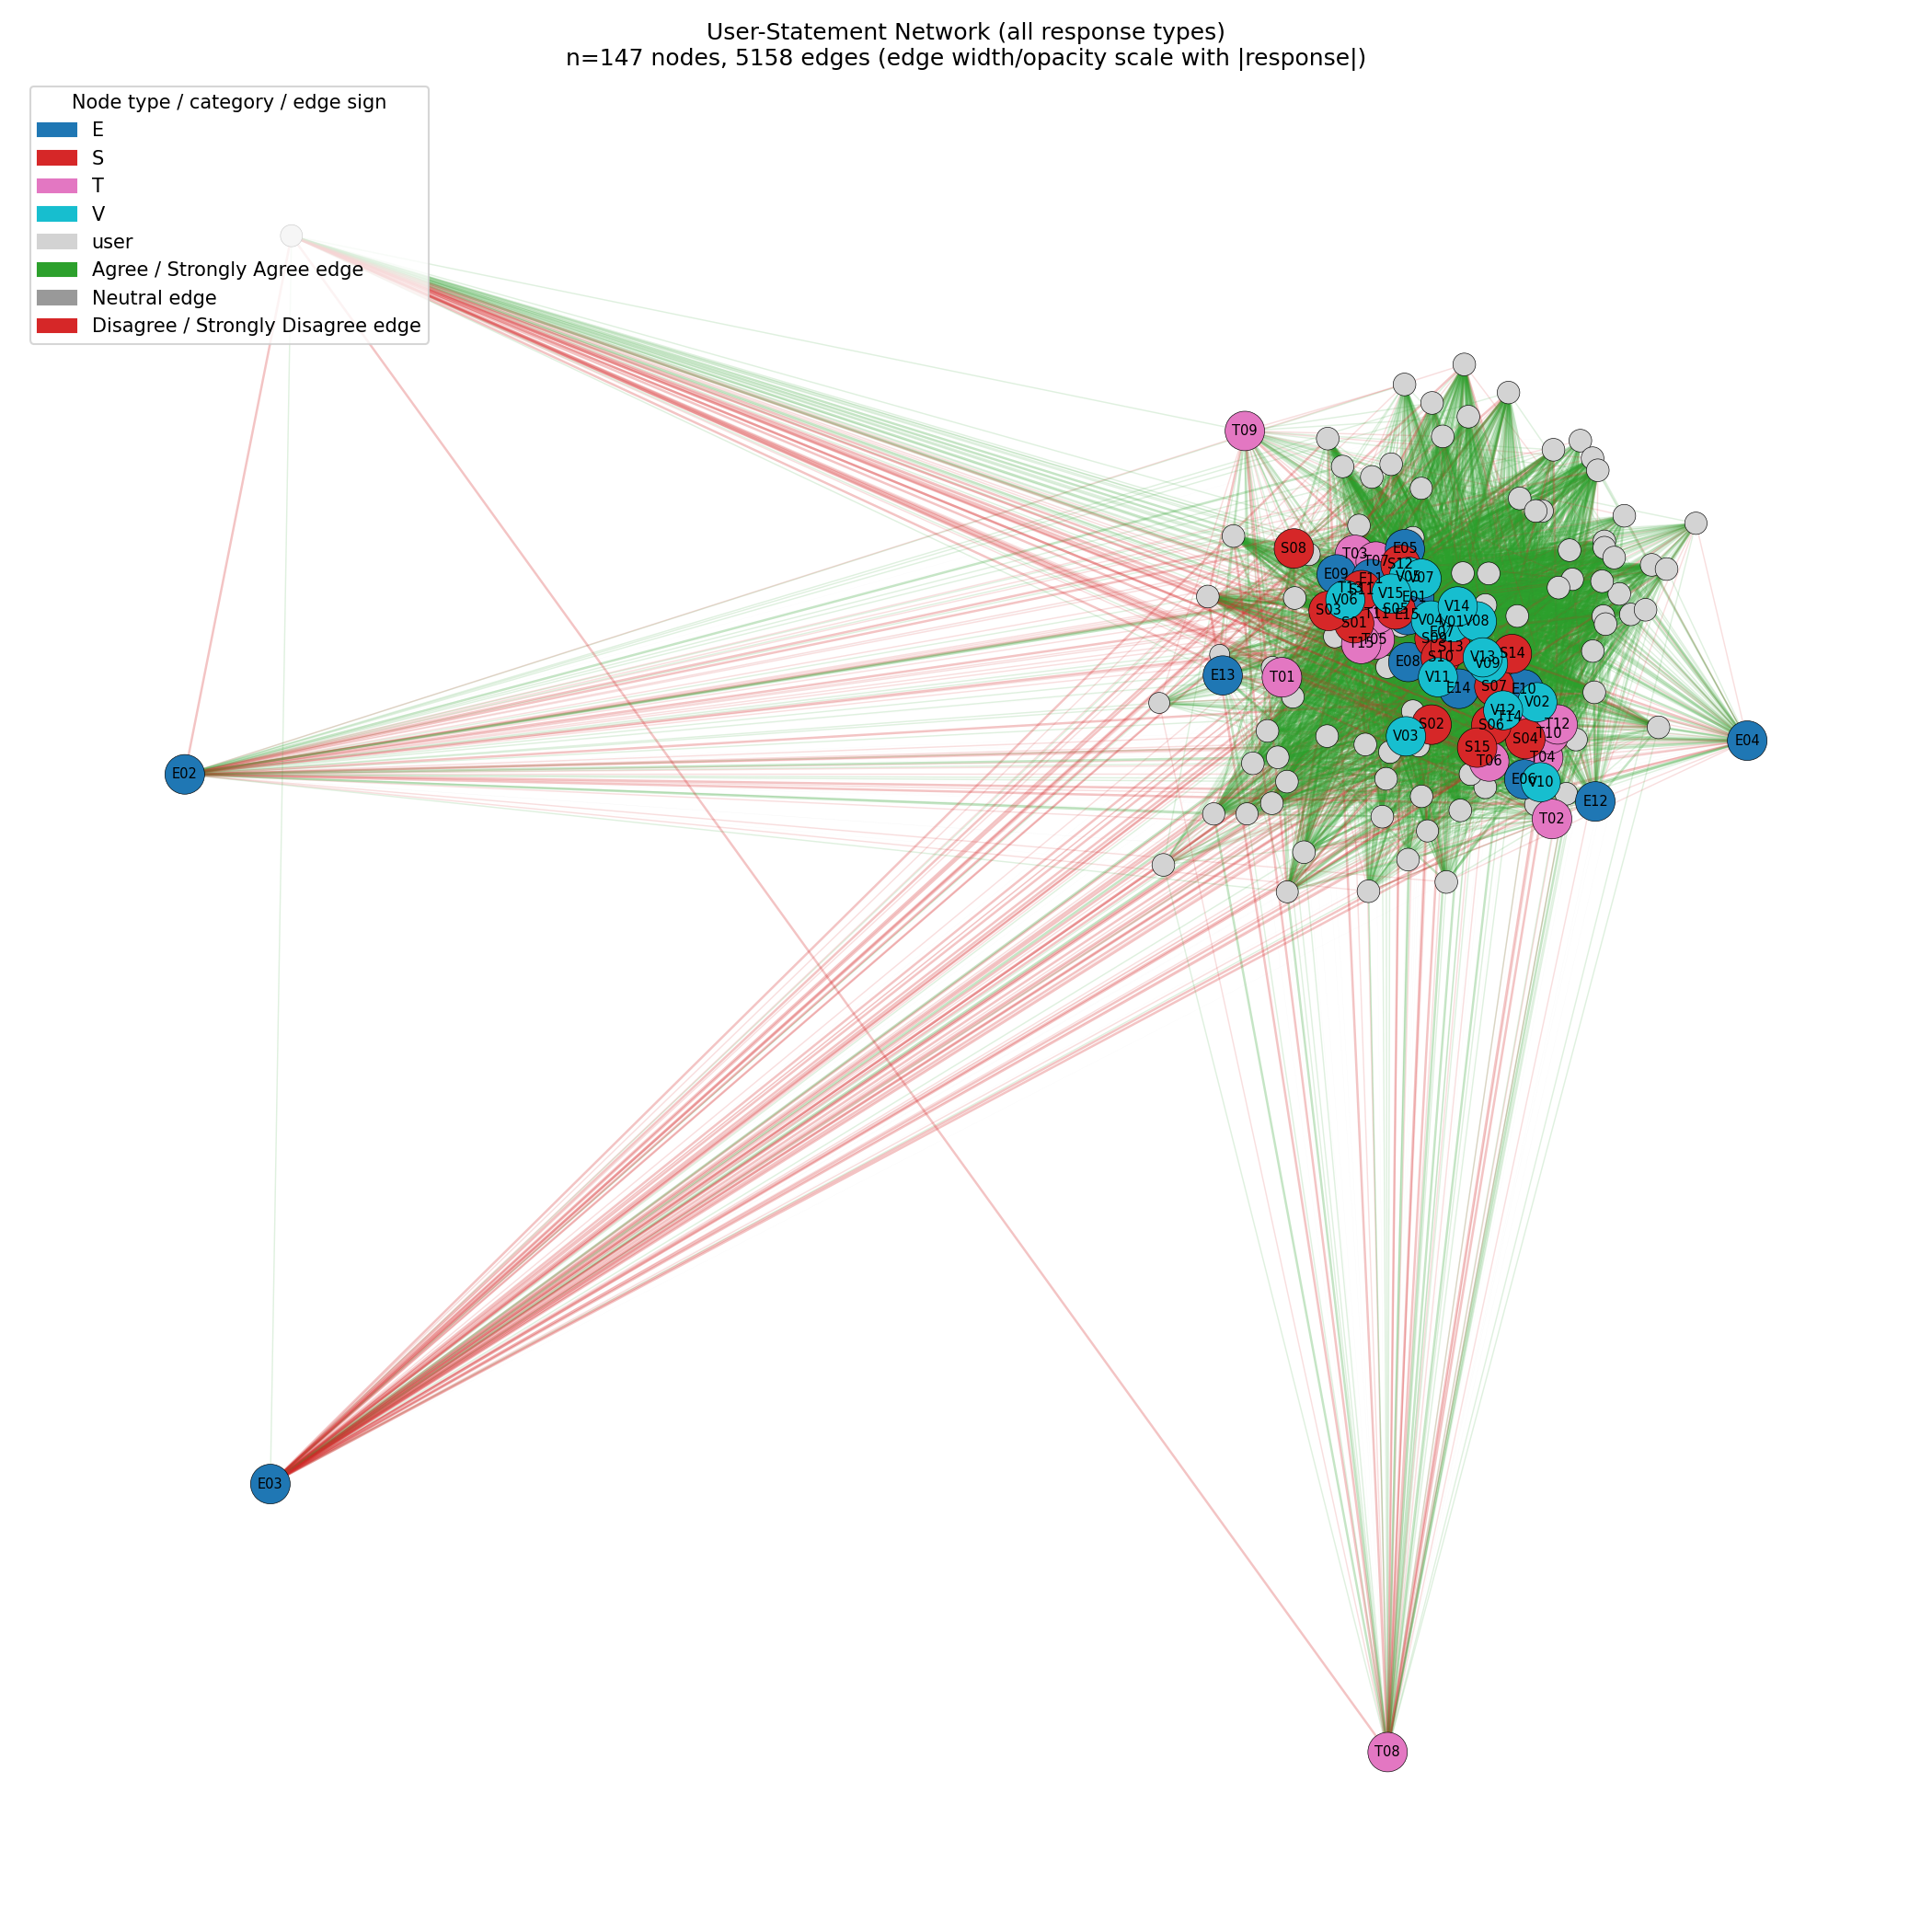
\includegraphics[width=0.47\textwidth]{../figures/user_statement_network.png}
    \caption{\textit{Left:} response heatmap (respondents sorted most disagreeable $\to$ most
    agreeable; statements grouped by category; 5 response colors + gray for missing).
    \textit{Right:} full bipartite network, all 5{,}158 edges and all five response types drawn
    (green = agree, red = disagree, gray = neutral; width/opacity $\propto |$weight$|$).}
    \label{fig:user-statement}
\end{figure}

\begin{center}
\begin{tabular}{lc}
\toprule
\textbf{Metric} & \textbf{Value} \\
\midrule
Users / Statements & 87 / 60 \\
Edges (answered) & 5{,}158 / 5{,}220 possible \\
Density $=|E|/(|U||S|)$ & 98.8\% \\
Mean edge weight $=\frac{1}{|E|}\sum_{(u,s)\in E} w_{u,s}$ & $+1.14$ \\
Response split & 80.0\% positive, 12.9\% neutral, 7.1\% negative \\
\bottomrule
\end{tabular}
\end{center}

Density near 100\% means missingness does not carry much structure here. Almost everyone answered
almost everything, so the real signal lives in edge \emph{weight} rather than edge presence. The
positive mean weight shows that the class leans toward agreement across the survey as a whole.

Per-node metrics: let $N(u) = \{s : (u,s)\in E\}$ (statements $u$ answered) and
$N(s) = \{u : (u,s)\in E\}$ (respondents who answered $s$), so $\deg(u)=|N(u)|$, $\deg(s)=|N(s)|$.

\begin{center}
\scriptsize
\begin{tabular}{p{2.9cm}p{4.6cm}p{6.1cm}}
\toprule
\textbf{Metric} & \textbf{Formula} & \textbf{What it tells us} \\
\midrule
mean\_response$(u)$ &
$\dfrac{1}{|N(u)|}\sum\limits_{s\in N(u)} w_{u,s}$ &
Respondent $u$'s average stance. Used to rank who is most agreeable and who is most disagreeable
overall. \\
\addlinespace
mean\_abs\_response$(u)$ &
$\dfrac{1}{|N(u)|}\sum\limits_{s\in N(u)} |w_{u,s}|$ &
Respondent $u$'s opinion \emph{intensity}, independent of direction. This separates decisive
respondents from wishy-washy ones (someone alternating between Strongly Agree and Strongly Disagree
scores high here even if their mean\_response is close to 0). \\
\addlinespace
mean\_response$(s)$ &
$\dfrac{1}{|N(s)|}\sum\limits_{u\in N(s)} w_{u,s}$ &
Statement $s$'s consensus level and direction (near $\pm2$ means broad agreement or disagreement,
near 0 means the respondents are split). \\
\addlinespace
std\_response$(s)$ &
$\sqrt{\dfrac{1}{|N(s)|-1}\sum\limits_{u\in N(s)} (w_{u,s}-\bar{w}_s)^2}$ &
Spread of opinion on $s$. A low std together with a high $|$mean$|$ points to a consensus statement,
while a high std points to a polarizing or contested statement, regardless of its average. \\
\bottomrule
\end{tabular}
\end{center}

By these metrics, consensus statements (high mean, low std) include E15 and V13, while the most
polarizing statements (high std) are E02, E03, and E04. It's worth noting that all three of the
polarizing ones come from the Education category.

% -----------------------------------------------------------------
\section{Results and Discussion}
% -----------------------------------------------------------------

\subsection{User--User Network}

\subsection{Statement--Statement Network}

\subsection{User--Statement Network}
The near-total density (98.8\%) combined with a positive mean edge weight ($+1.14$) shows the class
leans broadly toward agreement across the survey, consistent with the 80\%/13\%/7\%
positive/neutral/negative split (Section~5.3): most respondents answered most statements, and most
answers were Agree or Strongly Agree.

At the respondent level, mean\_response isolates a small set of genuine outliers from the agreeable
majority. Respondent 120 has the lowest mean\_response ($-0.21$), the only respondent whose average
stance falls on the disagreement side of neutral despite answering 56 of 60 statements. That looks
like a real dissenting voice rather than a low-engagement artifact.

At the statement level, std\_response identifies the Education-category statements E02, E03, and E04
as the most contested in the entire survey, while E15 and V13 are the strongest consensus statements.
It's worth pointing out that \textbf{S09}, the most structurally central statement in the
Statement--Statement network (highest degree and eigenvector centrality), also shows up among the
most consensus statements here (mean $1.47$, std $0.59$). So S09's centrality seems to come from
\emph{broad shared agreement} with many other statements rather than from controversy: centrality
and polarization are measuring two different things.

\subsection{Cross-Network Synthesis}

% -----------------------------------------------------------------
\section{Individual Contribution}
% -----------------------------------------------------------------

\begin{center}
\begin{tabular}{p{3cm}p{10cm}}
\toprule
\textbf{Member} & \textbf{Contribution} \\
\midrule
Name 1 & \\
\addlinespace
Name 2 & \\
\addlinespace
Priyanka Agarwal & User--Statement network: bipartite graph construction (\texttt{user\_statement\_network.py}), response-weighted edge scheme, per-user/per-statement metrics, heatmap and full-network visualizations, corresponding report sections. \\
\bottomrule
\end{tabular}
\end{center}

\end{document}
